\chapter{Experimental studies}
\label{sec:evaluation}

\textbf{Graph model:}
The road network or also known as spatial network is modeled as weighted graph where the crossroads are represented by nodes and roads are represented by the edges connecting the nodes. The weights on the edges in this specific research problem are the distances between the nodes on the edges. The distance between any two points can be found by summing up the lengths of the edges that belong to the shortest path between the two points.

\textbf{Dataset:}
The graph used to conduct the experiments on is constructed using Berlin's spatial datasets from \cite{datasets}, structured in separate CSV files for the crossroads, roads and points of interest. For the implementation of the operators the datasets are imported into a graph structure of nodes and edges, where each node has a unique id, its latitude and longitude and a list of PoIs that have been mapped to it and each edge has a source and destination node and the distance between the two nodes in kilometers as parameters. Each PoI is mapped to the nearest crossroad and has a unique id, a type, its latitude and longitude and the distance to the node it is mapped to.

The map used for the experiments is the road network of Berlin, with 428769 crossroad nodes, 504229 road edges, 5548 PoIs and 7 category types: restaurant, coffee shop, atms/bank, movie theater, pharmaciy, pubs/bar, gas station (see \ref{dataset}). 

\begin{table}[H]
	\centering
	\begin{tabular}{ |c|c|c| } 
		\hline
		\textit{Points} & \textit{Size} & \textit{Frequency}\\
		\hline
		Restaurants & 2081 & \multirow{3}{3em}{High}\\ 
		Coffee shops & 1002 &\\
		Pubs and bars & 958 &\\  
		\hline
		Atms/Banks & 597 & \multirow{3}{3em}{Middle}\\
		Pharmacies & 589 &\\
		\hline
		Gas stations & 180 & \multirow{3}{3em}{Low}\\
		Movie theaters & 141 &\\ 
		\hline
	\end{tabular}
	\caption{PoIs in Berlin's dataset}
	\label{dataset}
\end{table}

\textbf{Technical details:}
The experiments were performed on 2 Linux machines with AMD Opteron Processor 6212 with 2,60 GHz and Intel Xeon E5-2630 processor with 2.40GHz and respectively 16 CPUs and 128 GB RAM. The experiments for each parameter type were executed on 1000 queries with randomly selected starting points and the average of the results is reported.

Several experiments were conducted to evaluate the performance of the proposed algorithms. The evaluation criteria. which relate to all the operators, presented in the thesis are the following: (1) processing time (in milliseconds), (2) total number of heap fetches and (3) maximum heap size, representing the work space (WS) of the method.

\section{Equality operator}
\label{sec:experimentsEO}

The equality operator was evaluated with respect to the effect of following 3 parameters: (1) query length (cardinality of the category sequence $|M|$), (2) frequency of the categories in place of the equal indices i, j and (3) distance between the equal indices i, j in the category sequence $M$.

In the first set of experiments, shown in Figure \ref{fig:eo_length} a), b), c), the equality operator was evaluated in terms of query length, which varies from 3 to 7. Queries with length less than 3 would be immediately solved with PNE, which is why we do not consider them in these experiments. 
As we can see in Figure \ref{fig:eo_length} a), the query processing time increases proportionately to the query length. Figure \ref{fig:eo_length} a) also shows what portion of the total processing time of the proposed approach belongs to executing PNE in the first step of the algorithm. And as expected, both PNE's time and the proposed approach's time is increasing with the query length.
Figure \ref{fig:eo_length} b), c) follow the same trend of a). As query length increases, number of heap fetches and maximum heap size also increase.

\begin{figure}[H]
	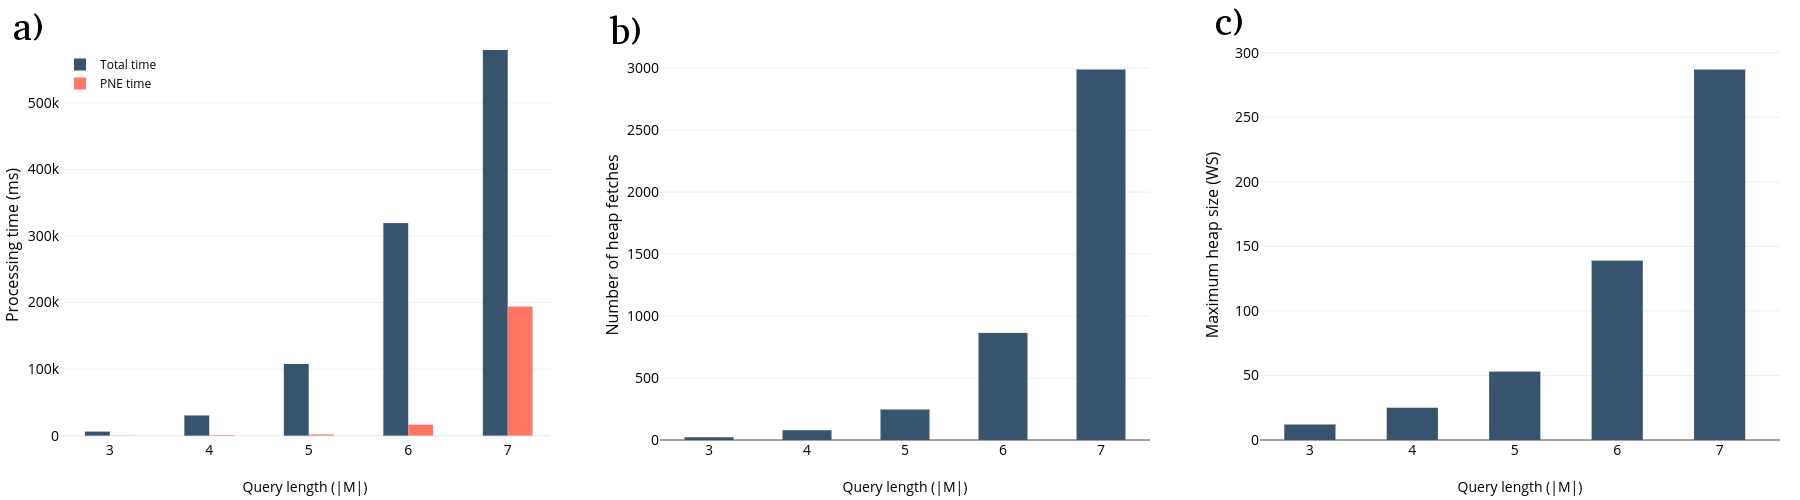
\includegraphics[scale=0.25]{images/eo_length.png}
	\centering
	\caption{Equality operator - query length experiments}
	\label{fig:eo_length}
\end{figure}

In the next set of experiments, shown in Figure \ref{fig:eo_frequency} a), b), c), the equality operator was evaluated in terms of the frequency of the categories in place of the equal indices i, j. Frequency relates to the size of each PoI dataset (see Table \ref{dataset}) and is categorized into low, middle and high, for a query length of 5.  Figure \ref{fig:eo_frequency} b), c) follow the same trend as the experiments for query length. 
As frequency of the categories, which are selected to be equal, increases, the processing time, number of heap fetches and heap maximum size increase proportionately. This can be explained with the fact that having more points in the PoI dataset of the equal categories increases the search space of the algorithm and respectively more partial routes are being generated, which increases the heap size, number of heap fetches and logically in turn the processing time.

\begin{figure}[H]
	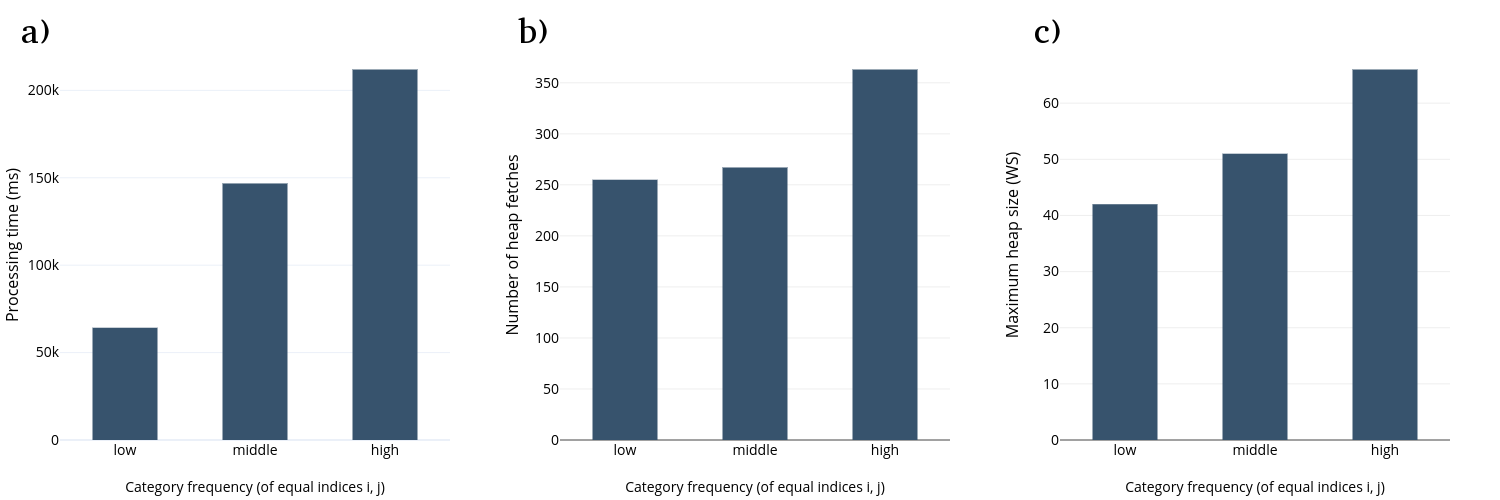
\includegraphics[scale=0.3]{images/eo_frequency.png}
	\centering
	\caption{Equality operator - category frequency experiments}
	\label{fig:eo_frequency}
\end{figure}

In the third set of experiments, shown in Figure \ref{fig:eo_distance} a), b), c), the equality operator was evaluated in terms of the  distance between the equal indices i, j in the category sequence $M$, which varies from 1 to 3, for a query length of 5. When the distance between the equal indices is 0, the result is always found with PNE, therefore we do not consider distance 1 in the experiments. 
As distance of the categories, which are selected to be equal, increases, the processing time, number of heap fetches and heap maximum size increase proportionately. This stems from the fact that by increasing the distance, the probability that the PoIs at indices i and j would be equal decreases, therefore less of the routes are found in the first step of the algorithm with PNE. This in turn causes the algorithm to continue with the heuristic approach in order to find an optimal route, which increases the processing time, number of heap fetches and also the work space (maximum heap size).

\begin{figure}[H]
	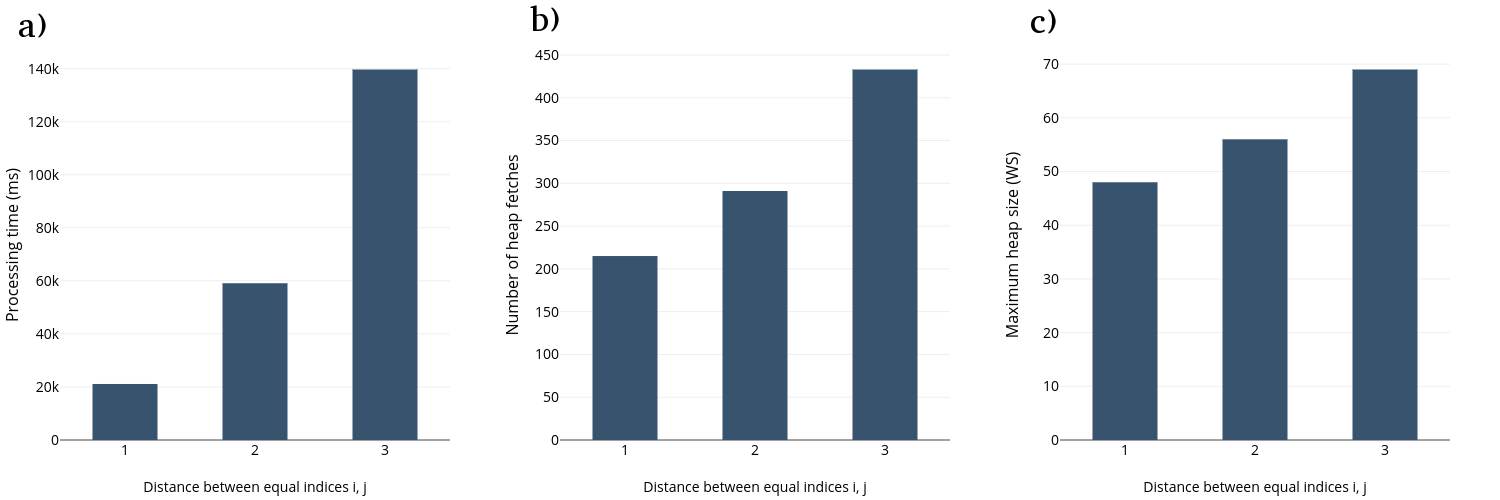
\includegraphics[scale=0.3]{images/eo_distance.png}
	\centering
	\caption{Equality operator - distance between equal indices experiments}
	\label{fig:eo_distance}
\end{figure}

Finally, the last set of experiments, shown in Figure \ref{fig:eo_distance} a), b), c), compare the baseline approach with the proposed approach in terms of query length. It can be seen that the proposed approach outperforms the baseline approach for all values of the query length. Also with increase in query length, the processing time , number of heap fetches and maximum heap size of the baseline approach increase with a rate that is more of that of the proposed approach, in \ref{fig:eo_distance} a) for query length 7 the processing time of the baseline approach is so long that it exceeds the graphic's range and is not fully depicted.

In conclusion, the proposed approach outperforms the baseline approach by a significant amount and it performs as expected in all parameters.

\begin{figure}[H]
	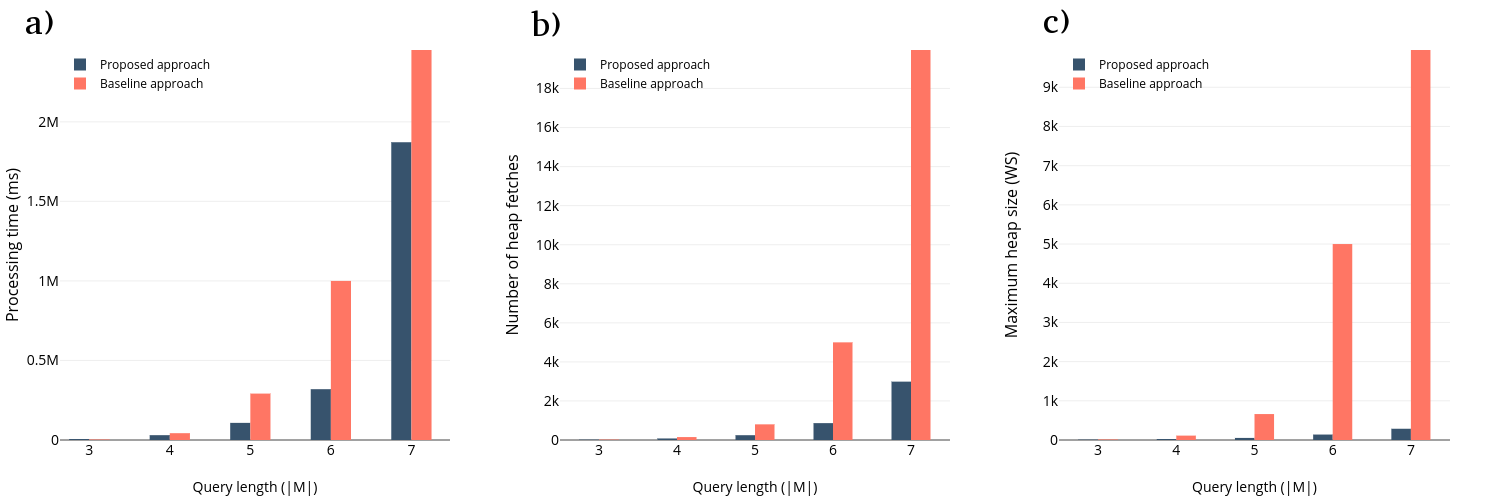
\includegraphics[scale=0.3]{images/eo2_length.png}
	\centering
	\caption{Equality operator - comparison between the proposed approach and the baseline approach}
	\label{fig:eo2_length}
\end{figure}


\section{Not-Equality operator}
\label{sec:experimentsNEO}

The not-equality operator was also evaluated with respect to the effect of following 3 parameters: (1) query length (cardinality of the category sequence $|M|$), (2) frequency of the categories in place of the equal indices i, j and (3) distance between the equal indices i, j in the category sequence $M$.

In the first set of experiments, shown in Figure \ref{fig:neo_length} a), b), c), the not-equality operator was evaluated in terms of query length, which varies from 3 to 7. As we can see in Figure \ref{fig:neo_length} a), the query processing time increases proportionately to the query length. Figure \ref{fig:neo_length} b), c) follow the same trend of a). As query length increases, number of heap fetches and maximum heap size also increase.

\begin{figure}[H]
	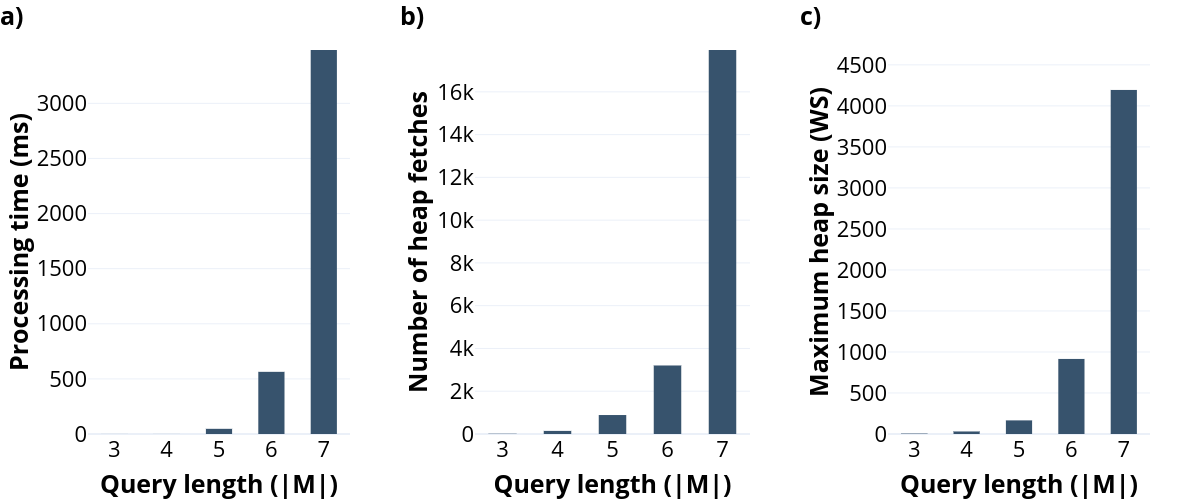
\includegraphics[scale=0.3]{images/neo_length.png}
	\centering
	\caption{Not-equality operator - query length experiments}
	\label{fig:neo_length}
\end{figure}

In the second set of experiments, shown in Figure \ref{fig:neo_frequency} a), b), c), the equality operator was evaluated in terms of the frequency of the categories in place of the equal indices i, j, which can be low, middle and high, for a query length of 5.  
Here we can see more interesting results than with the equality operator. The low frequency has higher results on all parameters than the middle frequency. This can be explained with the fact that when the categories which have to not be equal are less frequent, then the possibility of PNE reaching a route with different PoIs at places of the not equal categories is lower, therefore the not-equality algorithm searches for longer for not equal PoIs, compared to when the category has a middle frequency. And when the frequency is high, if PNE doesn't directly find a route with equal PoIs then the not-equality algorithm must inspect more points, therefore generates more routes and the time increases significantly. 
Figure \ref{fig:neo_frequency} b), c) follow the same trend as processing time.

\begin{figure}[H]
	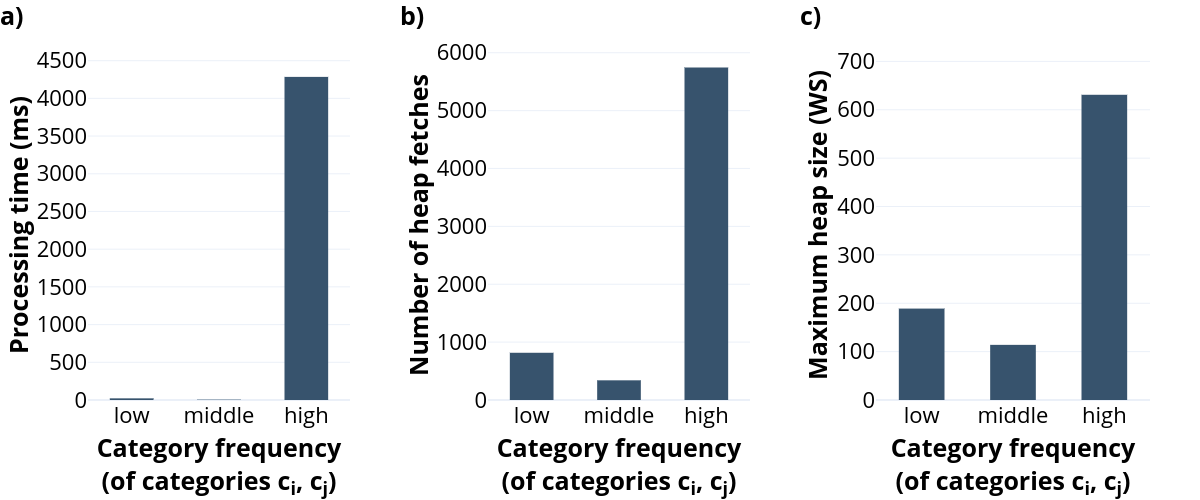
\includegraphics[scale=0.3]{images/neo_frequency.png}
	\centering
	\caption{Not-equality operator - category frequency experiments}
	\label{fig:neo_frequency}
\end{figure}

In the third set of experiments, shown in Figure \ref{fig:neo_distance} a), b), c), the equality operator was evaluated in terms of the  distance between the equal indices i, j in the category sequence $M$, which varies from 0 to 3, , for a query length of 5.  
Here we can also see more interesting results than with the equality operator. When the distance between the equal indices is 0, the result, usually found with PNE, always delivers equal points at indices i and j. Therefore the algorithm for the not-equality operator has to inspect more points in order to find the optimal route, where the PoIs at indices i and j are not equal to each other. This increases the search space and in turn the number of heap fetches, maximum heap size and the processing time increase as well. For distances 1, 2, 3 no obvious argumentation can be applied, because here we can not judge the possibility for equal PoIs found with PNE objectively.
% Is this argumentation okay?
Nevertheless, all three performance parameters - processing time, number of heap fetches and maximum heap size, follow the same trend and increase proportionately to each other.

\begin{figure}[H]
	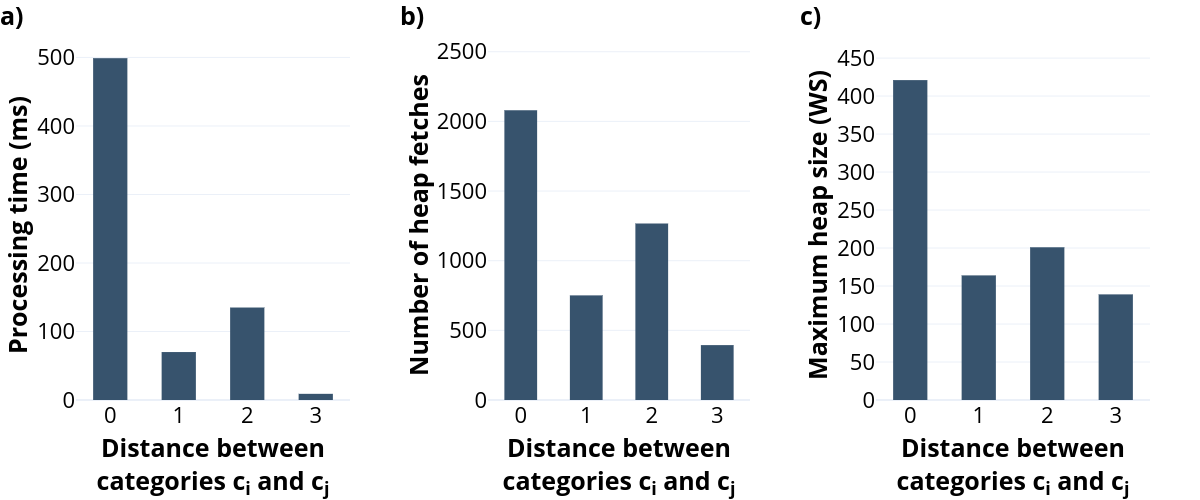
\includegraphics[scale=0.3]{images/neo_distance.png}
	\centering
	\caption{Not-equality operator - distance between not equal indices experiments}
	\label{fig:neo_distance}
\end{figure}


\section{Or operator}
\label{sec:experimentsOr}

The or operator was evaluated with respect to the type of number of operands, for a default query length of 5.  Three different types of queries were issued, where we changed the type and number of or operands in the first OR sequence $OR_1$ of the query, while the other four OR sequences only contained one category sequence with a single category. For 2 simple operands the first OR sequence contained two category sequenced with one single category each, for 3 simple operands the first OR sequence contained three category sequenced with one single category each and for 2 complex operands the first OR sequence contained two complex category sequences with 2 categories in each. In this way the complexity of the problem was gradually increased to see how the baseline approach compares to proposed approach of the algorithm.  
Figure \ref{fig:or} a), b), c) shows that the processing time, number of heap fetches and maximum heap size increase proportionately with the complexity of the query. As seen from the experiments the proposed approach is also by magnitudes faster and also more efficient in terms of heap size, as the complexity of the query increases. 

\begin{figure}[H]
	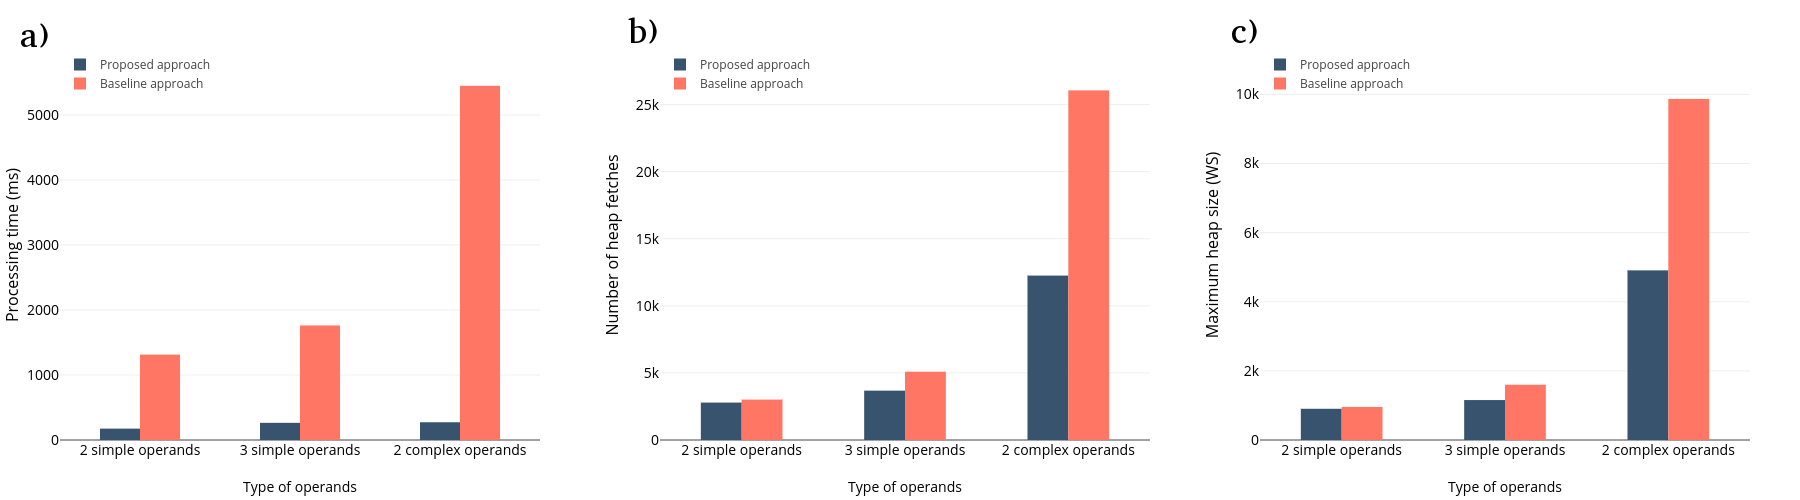
\includegraphics[scale=0.25]{images/or.png}
	\centering
	\caption{Or operator - type and number of operands experiments}
	\label{fig:or}
\end{figure}


\section{Order operator}
\label{sec:experimentsOrder}

The order operator was evaluated with respect to the number of fixed positions in a default query length of 5. The number ranges between 0 and 3. When the number of fixed positions is 4 or 5, the problem can be solved with simple PNE, therefore we do not consider these numbers in the experiments. The complexity of the problem is gradually decreased to see how the baseline approach compares to proposed approach of the algorithm.  
Figure \ref{fig:order} a), b), c) shows that the processing time, number of heap fetches and maximum heap size decrease proportionately with the complexity of the query. As seen from the experiments the proposed approach is also by magnitudes faster and also more efficient in terms of heap size.

\begin{figure}[H]
	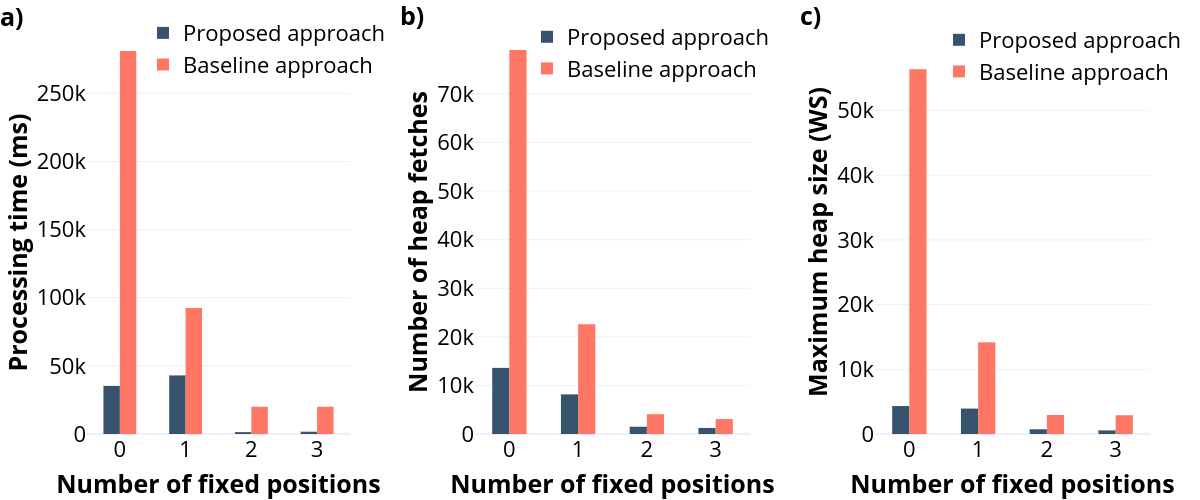
\includegraphics[scale=0.25]{images/order.png}
	\centering
	\caption{Order operator - number of fixed positions experiments}
	\label{fig:order}
\end{figure}

\section{Evaluation}
\label{sec:eval}
\todo{Todo: Evaluation}

%It is important to mention that the implemented approaches could be easily modified to return \textit{k} number of optimal routes, if the user may be interested
%Alternatives or additions to the route length: duration and PoI ratings

% We do not report I/O cost separately, because for all methods in all settings, the I/O time is no more than a few milliseconds; i.e., at least an order of magnitude lower than the total response time. 